\documentclass{birkjour}

\usepackage{amsmath}
\usepackage{amssymb}
\usepackage{amsthm}
\usepackage{graphicx}
\usepackage{float}
\usepackage{url}

\newtheorem{thm}{Theorem}[section]
 \newtheorem{cor}[thm]{Corollary}
 \newtheorem{lem}[thm]{Lemma}
 \newtheorem{prop}[thm]{Proposition}
 \theoremstyle{definition}
 \newtheorem{defn}[thm]{Definition}
 \theoremstyle{remark}
 \newtheorem{rem}[thm]{Remark}
 \newtheorem*{ex}{Example}
 \numberwithin{equation}{section}

\newcommand{\G}{\mathbb{G}}
\newcommand{\V}{\mathbb{V}}
\newcommand{\Vb}{\mathbb{\overline{V}}}
\newcommand{\W}{\mathbb{W}}
\newcommand{\R}{\mathbb{R}}
\newcommand{\B}{\mathbb{B}}

\newcommand{\Alpha}{A}
%\Omega is already defined

\newcommand{\nvao}{o}
\newcommand{\nvai}{\infty}
\newcommand{\nvaob}{\overline{o}}
\newcommand{\nvaib}{\overline{\infty}}

\newcommand{\eminus}{e_{-}}
\newcommand{\eplus}{e_{+}}
\newcommand{\eminusb}{\overline{e}_{-}}
\newcommand{\eplusb}{\overline{e}_{+}}

\begin{document}

\title{A Variation Of The Quadric Model\\Of Geometric Algebra}

\author{Spencer T. Parkin}
\email{spencer.parkin@gmail.com}

\numberwithin{equation}{section}

\subjclass{Primary 14J70; Secondary 14J29}

\keywords{Quadric Surface, Quartic Surface, Geometric Algebra, Quadric Model, Conformal Model}

%\dedicatory{To Melinda and Naomi}

\begin{abstract}
A variation of the quadric model set forth in \cite{Parkin12} is
found in which the rigid body motions are represented by
versors applicable to any quadric surface.
Extending this variation of the original model to include
a specific form of quartic surface, we find that these surfaces are
closed under the application of all conformal transformations.
Results of a computer program implementing this new model are presented.
\end{abstract}

\maketitle

\section{Introduction}

In the original paper \cite{Parkin12}, a model for quadric surfaces was
presented based upon the ideas of projective geometry.  What was unfortunate
about this model, however, was its lack of support for the rigid body transformations.  It was
predicted in the conclusion of that paper that a better model for quadric
surfaces may exist that is more like the conformal model of geometric algebra, here-after
abbreviated as CGA.
The present paper details what may be such a model.  We'll find that the rigid
body transformations can be incorporated into the model by using an alternative
method of encoding the quadric form.  An extension to this quadric form
will then allow us to support the conformal transformations at the expense of
expanding our model to necessarily include a specific form of quartic surfaces.  The
new model and its extension will both use the same geometric algebra to be given as follows.

\section{The Geometric Algebra}

We begin here with a description of the structure of the geometric algebra upon
which our model will be imposed.  This
geometric algebra will contain the following vector spaces.
\begin{equation}\label{equ_vector_spaces}
\begin{array}{ll}
\mbox{Notation} & \mbox{Basis} \\
\hline
\V^e & \{e_i\}_{i=1}^n \\
\V^{\nvao} & \{\nvao\}\cup\{e_i\}_{i=1}^n \\
\V^{\nvai} & \{e_i\}_{i=1}^n\cup\{\nvai\} \\
\V & \{\nvao\}\cup\{e_i\}_{i=1}^n\cup\{\nvai\}
\end{array}
\end{equation}
The set of vectors $\{e_i\}_{i=1}^n$ forms an orthonormal set of basis
vectors for the $n$-dimensional Euclidean vector space $\V^e$, which we'll
use to represent $n$-dimensional Euclidean space.
The vectors $\nvao$ and $\nvai$ are the familiar null-vectors representing the
points at origin and infinity, respectively, taken from CGA.
An inner-product table for these basis vectors is given as follows, where
$1\leq i<j\leq n$.
\begin{equation}
\begin{array}{c|cccc}
\cdot & \nvao & e_i & e_j & \nvai \\
\hline
\nvao & 0 & 0 & 0 & -1 \\
e_i & 0 & 1 & 0 & 0 \\
e_j & 0 & 0 & 1 & 0 \\
\nvai & -1 & 0 & 0 & 0
\end{array}
\end{equation}
We will now let $\G(\V)$ denote the Minkowski geometric algebra generated by $\V$.
For each vector space in table \eqref{equ_vector_spaces}, we will let an over-bar
above this vector space denote an identical copy of that vector space.  The vector
space $\W$ will denote the smallest vector space containing each of $\V$ and $\Vb$
as vector subspaces.  In symbols, one may write
\begin{equation}
\G(\W) = \G(\V\oplus\Vb).
\end{equation}

We will use over-bar notation to distinguish between vectors taken from $\V$
with vectors taken from $\Vb$.  Then, so that we may use the over-bar notation
in a well defined manner to distinguish between elements of $\G(\V)$ and $\G(\Vb)$,
we will define it as an outermorphic function that is also an isomorphism between
$\G(\V)$ and $\G(\Vb)$.  Doing so, we see that for any element $E\in\G(\V)$,
we may define $\overline{E}\in\G(\Vb)$ as
\begin{equation}
\overline{E} = SES^{-1},
\end{equation}
where $S$ is the versor given by
\begin{equation}\label{equ_isomorphism_versor}
S = (1+\eminus\eminusb)(1-\eplus\eplusb)\prod_{i=1}^n(1-e_i\overline{e}_i).
\end{equation}
This definition is non-circular if we let the over-bars in equation \eqref{equ_isomorphism_versor}
be purely notation.  The vectors $\eminus$ and $\eplus$, taken from \cite{LiRockwood},
are defined as
\begin{align}
\eminus &= \frac{1}{2}\nvai + \nvao, \\
\eplus &= \frac{1}{2}\nvai - \nvao.
\end{align}
The vectors $\eminusb$ and $\eplusb$ are defined similarly in terms of $\nvaob$ and $\nvaib$.
Defined this way, realize that, like the over-bar function defined in \cite{Parkin12},
here we have the property that for any vector $v\in\V$, we have $\overline{\overline{v}}=-v$.

\section{The Form Of Quadric Surfaces In $\G(\W)$}

We now give a formal definition under which elements $E\in\G(\W)$
are representative of $n$-dimensional quadric surfaces in our present variation
of the original model.
\begin{defn}\label{def_quadric}
Referring to an element $E\in\G(\W)$ as a quadric surface, it is representative of such an $n$-dimensional surface as the set of all points $p\in\V^o$ such that
\begin{equation}\label{equ_quadric_equation}
0 = p\wedge\overline{p}\cdot E.
\end{equation}
\end{defn}
From this definition it can be seen that the general form of a quadric $E\in\G(\W)$ is given by
\begin{equation}\label{equ_quadric_form}
E = \sum_{i=1}^k a_i\overline{b}_i,
\end{equation}
where each of $\{a_i\}_{i=1}^k$ and $\{b_i\}_{i=1}^k$ is a sequence of $k$ vectors
taken from $\V^\nvai$.  To see why, realize that the form \eqref{equ_quadric_form} can
always be reduced to the form
\begin{equation}\label{equ_quadric_reduced_form}
E \equiv \sum_{i=1}^n\sum_{j=i}^n\lambda_{ij}e_i\overline{e}_j+
\sum_{i=1}^n\lambda_i e_i\nvaib+
\lambda\nvai\nvaib,
\end{equation}
where each of $\lambda_{ij}$, $\lambda_i$, and $\lambda$ are scalars, in the
sense that this reduced form represents the same surface as that in equation \eqref{equ_quadric_form}
under Definition~\ref{def_quadric}.
We then see that this form \eqref{equ_quadric_reduced_form}, when it is
substituted into equation \eqref{equ_quadric_equation}, produces to a polynomial
equation of degree 2 in the vector components of $p-\nvao$.
Doing so with $p=\nvao+x$, where $x\in\V^e$, we get the equation
\begin{equation}\label{equ_quadric_polynomial_equation}
0 = -\sum_{i=1}^n\sum_{j=i}^n\lambda_{ij}(x\cdot e_i)(x\cdot e_j)
+\sum_{i=1}^n\lambda_i(x\cdot e_i) - \lambda,
\end{equation}
which we may recognize as the general equation of an $n$-dimensional quadric surface.

In practice, a computer program might take such a bivector of the form \eqref{equ_quadric_form}
and extract from it the coefficients of the quadric
polynomial \eqref{equ_quadric_polynomial_equation} it
represents.  It could then render the surface using traditional methods, such as those used
to render the traced surfaces in Figure~\ref{fig_invert_cylinder_in_sphere} far below.

Of course, using geometric algebra on paper, it might be undesirable and unnecessary to think of
quadrics in terms of polynomial equations.  A, perhaps, better way to think of quadrics is in terms
of an element of a geometric algebra whose decomposition
produces the parameters characterizing the quadric surface.  For example, many common
quadrics are the solution set in $\V^e$ of the equation
\begin{equation}
0 = -r^2 + (x-c)^2 + \lambda((x-c)\cdot v)^2,
\end{equation}
in the variable $x$.  (An explanation of the parameters $r$, $c$, $v$ and $\lambda$
was given in \cite{Parkin12}.)  Then, factoring out $-p\overline{p}$, we see that
the element $E\in\G(\W)$, given by
\begin{equation}\label{equ_canonical_form_of_common_quadric}
\Omega + \lambda v\overline{v}+2(c+\lambda(c\cdot v)v)\nvaib+
(c^2+\lambda (c\cdot v)^2-r^2)\nvai\nvaib
\end{equation}
is representative of this very same quadric by Definition~\ref{def_quadric},
where $\Omega$ is defined as
\begin{equation}
\Omega = \sum_{i=1}^n e_i\overline{e}_i.
\end{equation}
Canonical forms similar to \eqref{equ_canonical_form_of_common_quadric}
can be found for specific geometries, such as planes, spheres, plane-pairs,
circular cylinders, circular conical surfaces, and so on.

\section{Transformations Supported By The Model}

The main result of this section will depend upon the following lemma.
\begin{lem}\label{lma_versor_transfer}
For any versor $V\in\G(\W)$, and any four vectors $a,b,c,d\in\V$, we have
\begin{equation}
V^{-1}aV\wedge\overline{V^{-1}bV}\cdot c\wedge\overline{d} =
a\wedge\overline{b}\cdot V\overline{V}(c\wedge\overline{d})(V\overline{V})^{-1}.
\end{equation}
\end{lem}
\begin{proof}
We begin by first establishing that
\begin{align}
 & V^{-1}aV\wedge\overline{V^{-1}bV}\cdot c\wedge\overline{d} \\
=\;& -(V^{-1}aV\cdot c)(V^{-1}bV\cdot d) \\
=\;& -(a\cdot VcV^{-1})(b\cdot VdV^{-1}) \\
=\;& a\wedge\overline{b}\cdot VcV^{-1}\wedge\overline{VdV^{-1}}.
\end{align}
We now notice that
\begin{align}
& VcV^{-1} \\
=\;& V\overline{VV^{-1}}cV^{-1} \\
=\;& (-1)^m V\overline{V}c\overline{V^{-1}}V^{-1} \\
=\;& (-1)^m V\overline{V}c(V\overline{V})^{-1},
\end{align}
where $m$ is the number of vectors taken together in a geometric
product to form $V$.  We then notice that
\begin{align}
& \overline{VdV^{-1}} \\
=\;& VV^{-1}\overline{VdV^{-1}} \\
=\;& (-1)^{m^2}V\overline{V}V^{-1}\overline{dV^{-1}} \\
=\;&(-1)^{m^2+m}V\overline{Vd}V^{-1}\overline{V^{-1}} \\
=\;&(-1)^{2m^2+m}V\overline{VdV^{-1}}V^{-1} \\
=\;&(-1)^mV\overline{Vd}(V\overline{V})^{-1}.
\end{align}
It now follows that
\begin{equation}
a\wedge\overline{b}\cdot VcV^{-1}\wedge\overline{VdV^{-1}} =
a\wedge\overline{b}\cdot V\overline{V}(c\wedge\overline{d})(V\overline{V})^{-1}.
\end{equation}
\end{proof}
We're now ready to prove the main result as follows.
\begin{thm}\label{thm_quadric_transform}
Letting $E\in\G(\W)$ be a bivector of the form \eqref{equ_quadric_form},
$p,p'\in\V^o$ be a pair of points related by a versor $V\in\G(\V)$ by
the equation
\begin{equation}\label{equ_get_rid_ni}
p' = \nvao\cdot V^{-1}pV\wedge\nvai,
\end{equation}
and $E'\in\G(\W)$ a bivector given by
\begin{equation}\label{equ_transformed_surface}
E' = V\overline{V}E(V\overline{V})^{-1},
\end{equation}
the set of all points $p\in\V^\nvao$ such that
\begin{equation}\label{equ_wanted_variety}
0 = p'\wedge\overline{p}'\cdot E
\end{equation}
is exactly the set of all points $p\in\V^\nvao$ such that
\begin{equation}\label{equ_derived_variety}
0 = p\wedge\overline{p}\cdot E'.
\end{equation}
\end{thm}
\begin{proof}
The theorem goes through by the following chain of equalities.
\begin{align}
 & (\nvao\cdot V^{-1}pV\wedge\nvai)\wedge\overline{(\nvao\cdot V^{-1}pV\wedge\nvai)}\cdot E \\
=\;& V^{-1}pV\wedge\overline{V^{-1}pV}\cdot E \\
=\;& p\wedge\overline{p}\cdot(V\overline{V})E(V\overline{V})^{-1}.
\end{align}
The first equality holds by the fact that $E$ is of the form \eqref{equ_quadric_form},
while the second equality holds by Lemma~\ref{lma_versor_transfer}.
\end{proof}

The key motivation behind Theorem~\ref{thm_quadric_transform} is
the observation that the desired transformation of $E$ by $V$ is
given by the algebraic variety of equation \eqref{equ_wanted_variety}, because
an understanding of how $V^{-1}$ transforms $p$ gives us an understanding
of what type of geometry we get from equation \eqref{equ_wanted_variety} in terms of $E$ and $V$.
The theorem then
shows that this is also the algebraic variety of equation \eqref{equ_derived_variety}, thereby
giving us a means of performing desired transformations on elements representative
of quadric surfaces in $\G(\W)$, provided that $V$ is such a versor that $E'$ in
\eqref{equ_transformed_surface}, like $E$, is also a bivector of the form \eqref{equ_quadric_form}.
If this is not the case, then $V\overline{V}$ simply represents a transformation not
closed in the set of all quadric surfaces.

We can now apply Theorem~\ref{thm_quadric_transform} to show
that the rigid body transformations are supported in our new variation
of the original model.
Letting $\pi\in\V$ be a dual plane of CGA, given by
\begin{equation}
\pi = v+(c\cdot v)\nvai,
\end{equation}
where $v\in\V^e$ is a unit-length vector indicating the norm of the plane,
and where $c\in\V^e$ is a vector representing a point on the plane,
we see that for any homogenized point $p\in\V^o$, we have
\begin{equation}
-\pi p\pi^{-1} = \nvao+x-2((x-c)\cdot v)v + \lambda\nvai,
\end{equation}
where $p=\nvao+x$ with $x\in\V^e$, and
where the scalar $\lambda\in\R$ is of no consequence.  Letting $V=\pi$,
the point $p'\in\V^o$ of consequence here is given by equation \eqref{equ_get_rid_ni},
from which we can recognize an orthogonal reflection about the plane $\pi$.
It now follows by Theorem~\ref{thm_quadric_transform} that $\pi\overline{\pi}$ is a versor
capable of reflecting any quadric surface about the plane $\pi$.
Being able to perform planar reflections of any quadric in any plane, it
now follows that we can always find a versor $V\in\G(\W)$ capable of performing
any rigid body motion applicable to any quadric surface.  The development
of the rigid body motions, (combinations of translations and rotations), by planar reflections,
is well known, and can be found in section 2.7 of \cite{LiRockwood}.

Notice that not all versors of CGA are applicable in
our variation of the original quadric model.  This is because they fail to
satisfy the condition for closure that $E'$ be
of the form \eqref{equ_quadric_form}.

In retrospect, what we have done to find the rigid body motions
of quadric surfaces is similar to what was done in \cite{Langer08}; and
according to \cite{Pfister95}, we can state more generally that what we
have done is at least similar to finding an isomorphism between quadratic spaces.

\section{Extending The New Model}

\begin{figure}
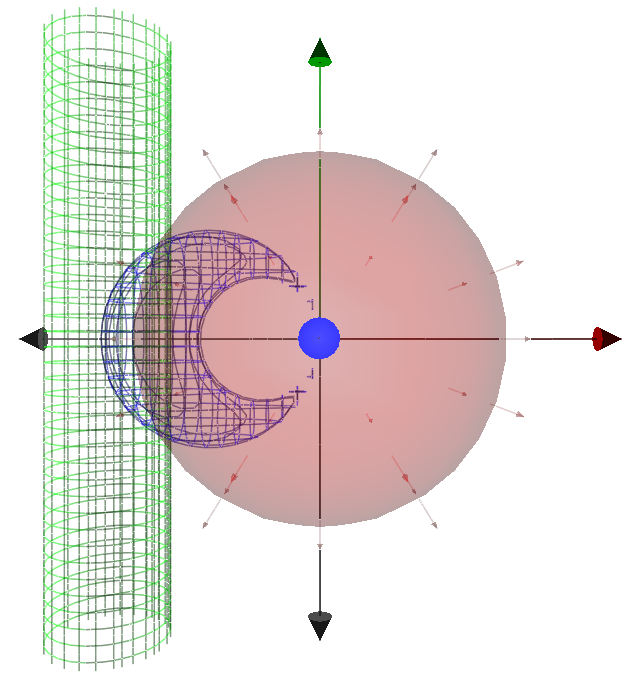
\includegraphics[scale=0.4]{InvertCylinderInSphere}
\caption{The inversion of a cylinder in a sphere.  Traces in various planes were
used to render the cylinder and its inversion.}
\label{fig_invert_cylinder_in_sphere}
\end{figure}
Interestingly, if we were not content with the rigid body motions of
quadrics, then we really could find what is, for example, the spherical
inversion of, say, an infinitely long cylinder in a sphere.  To do this, we change
Definition~\ref{def_quadric} into the following definition.
\begin{defn}\label{def_surface}
For any element $E\in\G(\W)$, we may refer to it as an $n$-dimensional
quartic surface as the set of all points $p\in\V^e$ such that
\begin{equation}\label{equ_surface_variety}
0 = P(p)\wedge\overline{P}(p)\cdot E,
\end{equation}
where $P:\V^e\to\V$ is the conformal mapping of CGA, defined in \cite{} as
\begin{equation}
P(p) = \nvao + p + \frac{1}{2}p^2\nvai.
\end{equation}
\end{defn}
A version of Theorem~\ref{thm_quadric_transform} is then easily found
such that if $V\in\G(\W)$ is any versor of CGA, and if $E$
is a surface under Definition~\ref{def_surface}, then the element $E'\in\G(\W)$,
given by equation \eqref{equ_transformed_surface}, must, by Definition~\ref{def_surface},
 be representative of the desired transformation of $E$ by the versor $V$.  The general
polynomial equation arising from the form of
such elements $E$ in Defintion~\ref{def_surface} is much more involved than
what we have in equation \eqref{equ_quadric_polynomial_equation}.  Nevertheless, it is possible to extract
a specific form of a quartic polynomial equation in
the vector components of $p$ from equation \eqref{equ_surface_variety}.
The result being unsightly, it will not be presented here.  Suffice it to say, a computerized
algebra system was used to find the polynomial form.  In any case, it is easy
to see from equation \eqref{equ_surface_variety} that the degree of the resulting
polynomial will be 4.

Now notice that under Definition~\ref{def_surface}, canonical forms
such as \eqref{equ_canonical_form_of_common_quadric} are still valid.
This is because
\begin{equation}
P(p)\wedge\overline{P}(p)\cdot E = (\nvao+p)\wedge\overline{(\nvao+p)}\cdot E
\end{equation}
in the case that $E$ is of the form \eqref{equ_quadric_form}.  This allows
us to use what we already know about quadrics in the new model with its extension.

Putting theory into practice, the author wrote a piece of computer
software that implements this CGA-like model for the special class of
quartic surfaces of equation \eqref{equ_surface_variety}.  Giving the program the following
script as input, the output of the program is given in Figure~\ref{fig_invert_cylinder_in_sphere}.
The script is easy for anyone to read, even if they are not familiar with its language.  It is given
here to illustrate how one might use the model with the aide a computer system.
%\begin{samepage}
{\small
\begin{verbatim}

/*
 * Calculate the surface that is the
 * inversion of a cylinder in a sphere.
 */
do
(
    /* Make the cylinder. */
    v = e2, c = -7*e1, r = 2,
    cylinder = Omega - v^bar(v) + 2*c*nib + (c.c - r*r)*ni^nib,
    bind_quadric(cylinder),
    geo_color(cylinder,0,1,0),
	
    /* Make the sphere. */
    c = 0, r = 6,
    sphere = no + c + 0.5*(c.c - r*r)*ni,
    bind_dual_sphere(sphere),
    geo_color(sphere,1,0,0,0.2),
	
    /* Make the inversion of the cylinder in the sphere. */
    V = sphere*bar(sphere),
    inversion = V*cylinder*V~,
    bind_conformal_quartic(inversion),
    geo_color(inversion,0,0,1),
)

\end{verbatim}
}
%\end{samepage}
The functions beginning with the word ``bind'' create and bind an entity to the given
element of the geometric algebra that is responsible for interpreting that element
as a surface under Definition~\ref{def_surface} or as a surface under the definition
given by CGA.  The computer program can then
use traditional methods to render the surface from the extracted polynomial equation.
For example, the polynomial equation in $x$, $y$ and $z$ for the inverted surface presented
in Figure~\ref{fig_invert_cylinder_in_sphere} is given by
\begin{equation}
\begin{split}
0 =\;& 28.8x^{2} + 11.2x^{3} + x^{4} + 11.2xy^{2} + 2x^{2}y^{2} + \\
 & 11.2xz^{2} + 2x^{2}z^{2} + y^{4} + 2y^{2}z^{2} + 28.8z^{2} + z^{4}.
\end{split}
\end{equation}
It is interesting how a bit of reasoning in geometric algebra has given us such a simple means
to obtaining this polynomial equation.
Of course, while such equations lend themselves to computer algorithms, they
are not practical on paper.  This is where the canonical forms of elements might become
useful; although, admittedly, even these forms have proven to be unwieldy
and impractical for the author, unlike their CGA counterparts.

\section{Closing Remarks}

The goal from the beginning has been to find a model, similar
to CGA, for the general set of surfaces up to degree 2,
not just the specific class of surfaces, up to degree 2, that are just the spheres and planes of CGA.
While this has been accomplished to some extent, one of the greatest deficiencies
remaining is the ability for the model to represent surfaces of up to the desired degree for
all dimensions from zero to $n$.
One possible solution, which is worth mentioning here at closing, is that of utilizing the geometric
algebra that is generated by the linear space of bivectors in $\G(\W)$.  We could
define a linear function on this space that maps it to a vector space $\B$.  If $f$ was such
a function, then for any pair of 2-blades $A,B\in\G(\W)$, we could define
\begin{equation}
f(A)\cdot f(B)=A\cdot B.
\end{equation}
It would then follow that a vector $v\in\G(\B)$ would be
representative of a surface as the set of all points $p\in\V^e$ such that
\begin{equation}
0 = \rho(p)\cdot v,
\end{equation}
where we define the function $\rho$ as
\begin{equation}
\rho(p) = f(P(p)\overline{P(p)}).
\end{equation}
The notions of dual and direct surfaces
would then emerge as they do in CGA.  We could then, using the outer product,
intersect dual surfaces and combine direct surfaces.  For a given versor $V\in\G(\V)$,
and a $k$-blade $B\in\G(\B)$, if we could find a vector factorization $v_1\wedge\dots\wedge v_k$
of $B$, then the transformation $B'$ of $B$ by $V$ would be given by
\begin{equation}
B' = \bigwedge_{i=1}^k f(V\overline{V}f^{-1}(v_i)(V\overline{V})^{-1}).
\end{equation}
See \cite{} on the problem of blade factorization.  It is unfortunate that we would
have to bother finding such a factorization to transform a surface.

To illustrate the use of $\G(\B)$, let $s,c\in\G(\B)$ be vectors dually representative
of a sphere and cylinder, respectively.  Then, for any point $p\in\V^e$, we can find
the dual surface containing $p$ and the intersection of $s$ and $c$ as
\begin{equation}\label{equ_pencil}
(\rho(p)\wedge(s\wedge c)I)I = \rho(p)\cdot s\wedge c = (\rho(p)\cdot s)c - (\rho(p)\cdot c)s,
\end{equation}
where $I$, in practice, might be the unit psuedo-scalar of the geometric algebra
generated by the vector sub-space of $\B$ given by the set
\begin{equation}
\{f(x\overline{y})|x,y\in\V\}.
\end{equation}
Even this vector space, which is of dimension $(n+2)^2$, is larger than it needs to be.
We could suffice with a vector space of dimension $(n+2)(n+3)/2$.
In any case, it is clear from equation \eqref{equ_pencil} that the algebra
is simply giving us the desired surface in the pencil of $s$ and $c$.

Unlike CGA, however, even in our use of $\G(\B)$, there does not appear
to be any easy way to perform geometric analysis on given geometries.
For example, in CGA, a given element can always be decomposed into
a set of parameters characterizing the geometry by interpreting that
element in terms of a known canonical form.  (The intersection of two
spheres may be interpreted as the intersection of a sphere centered on a plane.)
There does not appear to be any easy equivalent of this idea in $\G(\B)$ in all cases,
and so we must defer to the literature, such as \cite{} and \cite{}, to learn
anything interesting about a given dual surface of dimension less than $n$.

\nocite{Dorst07}
\bibliographystyle{amsplain}
\bibliography{Parkin_AVariationOfTheQuadricModelOfGA}

% cite http://www.math.ethz.ch/~knus/papers/campinas.pdf -> quad forms determine clifford algebras?
% cite http://www.maths.ed.ac.uk/~aar/books/dublin.pdf for history of quadratic forms
% cite wiki entry for algebraic variety?

\end{document}